\documentclass[11pt,a4paper]{article}

% ---------- Packages ----------
\usepackage[utf8]{inputenc}
\usepackage[T1]{fontenc}
\usepackage[margin=2.5cm]{geometry}
\usepackage{float}
\usepackage{tikz}
\usetikzlibrary{shapes.geometric,arrows.meta,positioning,fit,backgrounds,calc,decorations.pathreplacing}
\usepackage{booktabs}
\usepackage{xcolor}
\usepackage{titlesec}
\usepackage{fancyhdr}
\usepackage{hyperref}
\usepackage{enumitem}
\usepackage{parskip}
\usepackage{caption}
\usepackage{amsmath}

% ---------- Colors ----------
\definecolor{cplane}{RGB}{28,63,107}     % C data plane / hardware
\definecolor{pyplane}{RGB}{31,110,92}    % Python control plane
\definecolor{gapbox}{RGB}{150,60,50}     % undocumented subsystem
\definecolor{neutralbox}{RGB}{70,70,70}
\definecolor{lightbg}{RGB}{245,247,250}

% ---------- Header/Footer ----------
\pagestyle{fancy}
\fancyhf{}
\renewcommand{\headrulewidth}{0.3pt}
\fancyhead[L]{\small Edge Spectrum Sensor --- Architecture Reference}
\fancyhead[R]{\small\thepage}
\fancyfoot[C]{\small Conceptual and Methodological Reference (No Source Code)}

\titleformat{\section}{\normalfont\Large\bfseries\color{cplane}}{\thesection}{0.6em}{}
\titleformat{\subsection}{\normalfont\large\bfseries}{\thesubsection}{0.6em}{}

\hypersetup{
    colorlinks=true,
    linkcolor=cplane,
    citecolor=cplane,
    urlcolor=pyplane
}

\newcommand{\undoc}[1]{\textcolor{gapbox}{\textit{#1}}}

\title{
    \vspace{-1.5cm}
    {\Large\bfseries Architecture Reference for an Edge-Based\\ RF Spectrum Sensing Node}\\[0.3cm]
    {\large A Conceptual and Methodological Description of a\\ Raspberry~Pi~5 / HackRF~One / GPS-LTE / RF-Multiplexer Sensor}
}
\author{Prepared for internal research review}
\date{\today}

\begin{document}
\maketitle
\thispagestyle{fancy}

\begin{abstract}
\noindent
This document describes, at the conceptual and methodological level, the architecture of an
edge-deployed radio-frequency (RF) spectrum sensing node built around a Raspberry~Pi~5 host,
a HackRF~One software-defined radio (SDR) front end, an RF multiplexer for antenna-port
selection, and a GPS/LTE module for geolocation, time reference, and backhaul connectivity.
The system is designed as a dual-plane architecture: a real-time \emph{data plane} implemented
in C, responsible for IQ acquisition and digital signal processing (DSP) under bounded latency,
and a supervisory \emph{control plane} implemented in Python, responsible for scheduling,
telemetry, and communication with a remote coordination server. We describe the design
principles that govern the separation of these planes, the methodologies used for spectral
estimation, calibration, fault recovery, and data integrity, and we position the system
relative to existing state-of-the-art (SOTA) distributed spectrum-sensing platforms. Where
a subsystem is known to exist and to be operationally load-bearing but is not documented in
the source material available to the authors of this reference --- specifically the internal
design of the GPS/LTE engine and the RF multiplexer --- we describe only its externally
observable interface contract and explicitly flag the internal mechanism as undocumented,
rather than inferring implementation detail that cannot be verified.
\end{abstract}

\tableofcontents

% =====================================================================
\section{Introduction and Context}
% =====================================================================

\subsection{Motivation}

Wide-area radio spectrum monitoring has traditionally relied on a small number of expensive,
professionally operated monitoring stations. Regulatory bodies responsible for spectrum
management --- allocating frequency bands, detecting interference, and enforcing licensed use
--- have historically been constrained by the cost and limited geographic density of such
stations. Over the last decade, the falling cost of software-defined radio front ends and
single-board computers has made it feasible to deploy larger numbers of lower-cost, unattended
sensing nodes at the network edge, trading some per-node measurement fidelity for spatial
density, deployment flexibility, and continuous operation.

The system described here follows this edge-sensing paradigm. It is designed to run
unattended for extended periods, to report both scheduled (``campaign'') and on-demand
(``realtime'') spectral measurements to a remote coordination server, and to do so within the
power, thermal, and compute envelope of a single-board computer.

\subsection{Related Work and State of the Art}

Distributed, low-cost spectrum sensing has an established research and deployment lineage.
Platforms such as \textbf{ElectroSense} demonstrated that a Raspberry~Pi paired with a
low-cost SDR front end (originally RTL-SDR-class hardware, later extended with
up/down-converters to reach into the low-GHz range) could be crowdsourced into a distributed
sensing network with a shared backend and open API, performing on-device FFT-based feature
extraction before streaming measurements to a cloud backend. Its successor,
\textbf{ElectroSense+}, moved further processing to the edge and added encrypted remote-access
and user-controlled demodulation services, illustrating a broader trend in the field: as edge
compute capacity grows, more of the DSP burden migrates from the cloud back to the sensor
itself, reducing backhaul bandwidth and enabling lower-latency local decisions (e.g.,
DC-spike removal, channel filtering, or modulation-quality estimation) before data ever
leaves the node. Related distributed-sensing efforts (e.g., SpecSense-class systems, and
IoT-oriented spectrum cartography research) share a common architectural skeleton: an
inexpensive embedded compute platform, an SDR front end, a local acquisition/DSP stage, and
a scheduling/reporting layer that talks to a central server.

The system described in this reference sits within that same lineage but differs from the
canonical crowdsourced model in three respects that are methodologically significant:

\begin{enumerate}[leftmargin=1.4em]
    \item \textbf{Regulatory rather than crowdsourced operation.} The node reports to a
    single authoritative coordination server rather than a public crowdsourcing backend,
    and supports scheduled regulatory ``campaigns'' with defined time windows in addition
    to ad-hoc realtime queries.
    \item \textbf{A higher-performance, wider-range SDR front end.} HackRF~One provides
    continuous tuning from below 1~MHz to 6~GHz at up to 20~Msps, removing the need for an
    auxiliary up/down-converter that RTL-SDR-class front ends typically require to reach
    the same range.
    \item \textbf{A hard split between a real-time data plane and a supervisory control
    plane}, implemented in different languages and processes, communicating over a local
    IPC channel rather than being organized as a single monolithic acquisition process.
    This is discussed at length in Section~\ref{sec:methodology}.
\end{enumerate}

\subsection{Scope of This Document}

This is a conceptual and methodological reference. It does not reproduce source code,
function signatures, or file-level implementation detail; it describes \emph{what the system
does, why it is structured the way it is, and which design patterns are used to satisfy which
requirements}. Where a component's internal design is not available in the documentation
this reference was derived from, that gap is stated explicitly rather than filled by
inference.

% =====================================================================
\section{System Overview}
% =====================================================================

The sensor node integrates four physical subsystems and two logical software planes on a
single embedded host. Figure~\ref{fig:stack} shows the system as a vertical stack, from the
remote coordination server down to the antenna.

\begin{figure}[h]
\centering
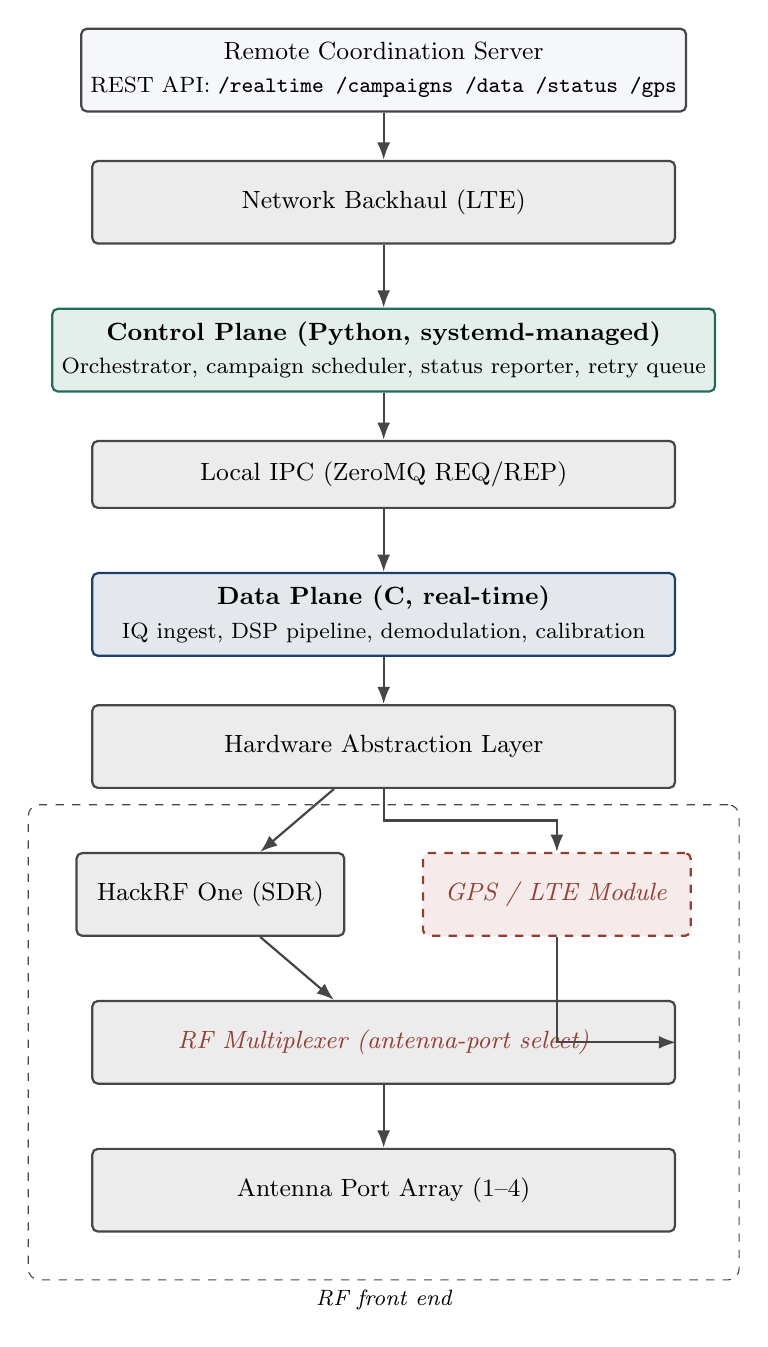
\begin{tikzpicture}[
    node distance=6mm,
    box/.style={rectangle, rounded corners=2pt, draw=neutralbox, thick,
                minimum width=7.4cm, minimum height=1.05cm, align=center,
                font=\small},
    cbox/.style={box, fill=cplane!12, draw=cplane},
    pybox/.style={box, fill=pyplane!12, draw=pyplane},
    hwbox/.style={box, fill=neutralbox!10, draw=neutralbox},
    gbox/.style={box, fill=gapbox!10, draw=gapbox, dashed},
    arr/.style={-{Latex[length=2.2mm]}, thick, neutralbox}
]

\node[box, fill=lightbg] (server) {Remote Coordination Server\\[1pt]{\footnotesize REST API: \texttt{/realtime /campaigns /data /status /gps}}};

\node[hwbox, below=of server] (net) {Network Backhaul (LTE)};

\node[pybox, below=8mm of net] (orch) {\textbf{Control Plane (Python, systemd-managed)}\\[1pt]{\footnotesize Orchestrator, campaign scheduler, status reporter, retry queue}};

\node[hwbox, below=of orch, minimum height=0.85cm] (ipc) {Local IPC (ZeroMQ REQ/REP)};

\node[cbox, below=8mm of ipc] (rfengine) {\textbf{Data Plane (C, real-time)}\\[1pt]{\footnotesize IQ ingest, DSP pipeline, demodulation, calibration}};

\node[hwbox, below=of rfengine] (hal) {Hardware Abstraction Layer};

\node[hwbox, below=8mm of hal, minimum width=3.4cm, xshift=-2.2cm] (hackrf) {HackRF One (SDR)};
\node[gbox, below=8mm of hal, minimum width=3.4cm, xshift=2.2cm] (gpslte) {\undoc{GPS / LTE Module}};

\node[hwbox, below=8mm of hackrf, xshift=2.2cm, minimum width=7.4cm] (mux) {\undoc{RF Multiplexer (antenna-port select)}};

\node[hwbox, below=8mm of mux, minimum width=7.4cm] (ant) {Antenna Port Array (1--4)};

\draw[arr] (server) -- (net);
\draw[arr] (net) -- (orch);
\draw[arr] (orch) -- (ipc);
\draw[arr] (ipc) -- (rfengine);
\draw[arr] (rfengine) -- (hal);
\draw[arr] (hal) -- (hackrf);
\draw[arr] (hal.south) -- ++(0,-4mm) -| (gpslte.north);
\draw[arr] (hackrf) -- (mux);
\draw[arr] (gpslte) |- (mux);
\draw[arr] (mux) -- (ant);

\begin{scope}[on background layer]
\node[fit=(hackrf)(gpslte)(mux)(ant), draw=neutralbox, dashed, inner sep=6mm, rounded corners=4pt, label={[font=\footnotesize\itshape]below:RF front end}] {};
\end{scope}

\end{tikzpicture}
\caption{Vertical system stack. Solid blue/green boxes are documented in detail; dashed red
boxes (GPS/LTE module, RF multiplexer) are known to exist and to be operationally used, but
their internal design is not covered by the available documentation --- only their externally
observable interface contract is known (see Section~\ref{sec:gpslte}).}
\label{fig:stack}
\end{figure}

The host operating system schedules the two software planes as independent, restart-supervised
processes. This separation is the central methodological choice of the system and is discussed
next.

% =====================================================================
\section{Design Methodology and Principles}
\label{sec:methodology}
% =====================================================================

Five principles recur throughout the system and can be treated as the design methodology
against which individual components should be evaluated.

\subsection{Data-Plane / Control-Plane Separation}

The system draws a hard boundary between code that must meet real-time deadlines (sample
ingestion, DSP, hardware register access) and code that governs longer-horizon decisions
(what to measure, when, and where to send it). The former is implemented in C, compiled to a
native binary, and given real-time-adjacent scheduling considerations (thread affinity
avoidance, passive wait policies). The latter is implemented in Python as a set of
independently restartable services. The two communicate over a single, narrow, well-defined
local IPC contract (request/reply, JSON-encoded) rather than sharing memory or process space.

The methodological benefit of this split is fault isolation: a defect or crash in the
orchestration logic (scheduling, HTTP retry policy, telemetry formatting) cannot corrupt or
stall the acquisition hot path, and a hardware-level fault in the SDR driver cannot bring down
the process responsible for talking to the coordination server. Each plane can also be
restarted independently by the service supervisor without requiring the other to reinitialize.

\subsection{Hardware Arbitration via a Global State Machine}

Because the SDR front end is a single physical resource, the system enforces mutual exclusion
over acquisition activity at the control-plane level through a global state machine with a
small number of mutually exclusive states (idle, on-demand/realtime acquisition, scheduled
campaign acquisition, calibration). This is a coarse-grained but effective concurrency
control mechanism: rather than relying on low-level locking around the hardware driver, the
system prevents conflicting acquisition intents from ever being issued in the first place.
Section~\ref{sec:statemachine} describes this model in more detail.

\subsection{Request-Scoped Acquisition Semantics}

Every acquisition is scoped to the request that triggered it. Before capturing samples for a
given request, any data buffered prior to that request is discarded, so that the response is
guaranteed to reflect spectrum conditions \emph{after} the request was issued rather than
stale, pre-existing buffer contents. This is a subtle but important correctness property for
a system whose clients (regulatory operators, scheduled campaigns) expect a measurement to
correspond to a specific point in time, not to whatever happened to be sitting in a buffer.

\subsection{Fault Containment and Self-Healing}

The system is designed on the assumption that most of its failure modes are transient:
USB/SDR disconnects, IPC socket desynchronization, network timeouts, and thermal or power
fluctuations typical of unattended field deployment. The methodology favors automatic,
bounded-retry self-healing over operator intervention:
\begin{itemize}[leftmargin=1.4em]
    \item IPC channels that enter an inconsistent state (e.g., a stalled request/reply
    handshake) are torn down and recreated rather than nursed back to a known state.
    \item Hardware sessions are health-checked before use and invalidated/reopened on
    failure, with a bounded number of recovery attempts.
    \item Long-running worker threads and processes check a cancellation flag on a short
    polling interval so that shutdown and recovery remain responsive even mid-operation.
    \item Process-level supervision (restart-always policies with lock-guarded singleton
    enforcement) forms the outermost layer of defense against unrecoverable in-process
    failures.
\end{itemize}

\subsection{Persistence and Atomicity}

State that must survive process restarts or be shared between the data plane and the control
plane (e.g., calibration results, GPS fix, campaign lock flags) is written to a shared,
memory-backed store using an atomic write discipline: write to a temporary location, flush,
then atomically replace the target, under an advisory lock that distinguishes shared
(read) from exclusive (write) access. This avoids partial-write corruption if the node loses
power or a process is killed mid-write, which is a realistic occurrence for unattended,
field-powered equipment.

% =====================================================================
\section{Subsystem Architecture}
% =====================================================================

\subsection{RF Data Plane}

The data plane's job is to turn a stream of raw IQ samples into either a spectral estimate or
a demodulated audio stream, within bounded latency, on a single-board computer's compute
budget. Conceptually it is organized as a pipeline (Figure~\ref{fig:dsp}):

\begin{enumerate}[leftmargin=1.4em]
    \item \textbf{Ingest.} Samples are handed off from the SDR driver's callback context into
    a lock-free, single-producer/single-consumer circular buffer. This decouples the
    high-frequency hardware callback from the consumer(s) reading from it, so that neither
    can block the other.
    \item \textbf{Signal conditioning.} Raw samples are converted to a normalized complex
    representation and corrected in place for DC offset, and I/Q gain and phase imbalance ---
    endemic front-end impairments in direct-conversion SDR hardware that would otherwise
    distort spectral estimates.
    \item \textbf{Optional channel isolation.} When a request specifies a sub-band of
    interest, a frequency-domain filter isolates it prior to further processing, using a
    two-stage approach: an outlier-clipping stage to prevent strong out-of-band interferers
    from dominating the result, followed by a smooth-transition (raised-cosine) masking
    stage chosen specifically to minimize time-domain ringing artifacts.
    \item \textbf{Spectral estimation or demodulation.} Depending on the request, the
    conditioned signal is either passed through a power spectral density (PSD) estimator
    (two interchangeable methods are supported, trading estimation quality against
    computational cost) or through an FM/AM demodulation chain that also derives simple
    modulation-quality metrics (deviation, depth) as a byproduct.
    \item \textbf{Publish.} Results are serialized and returned over the same request/reply
    channel the request arrived on.
\end{enumerate}

A concurrent, independently running audio path drains a secondary buffer continuously
(rather than per-request) whenever demodulation is active, encodes PCM audio into a
compressed frame format, and streams it out over a separate network channel --- allowing a
human operator to listen to a demodulated signal while spectral requests continue to be
served on the primary path.

\begin{figure}[H]
\centering
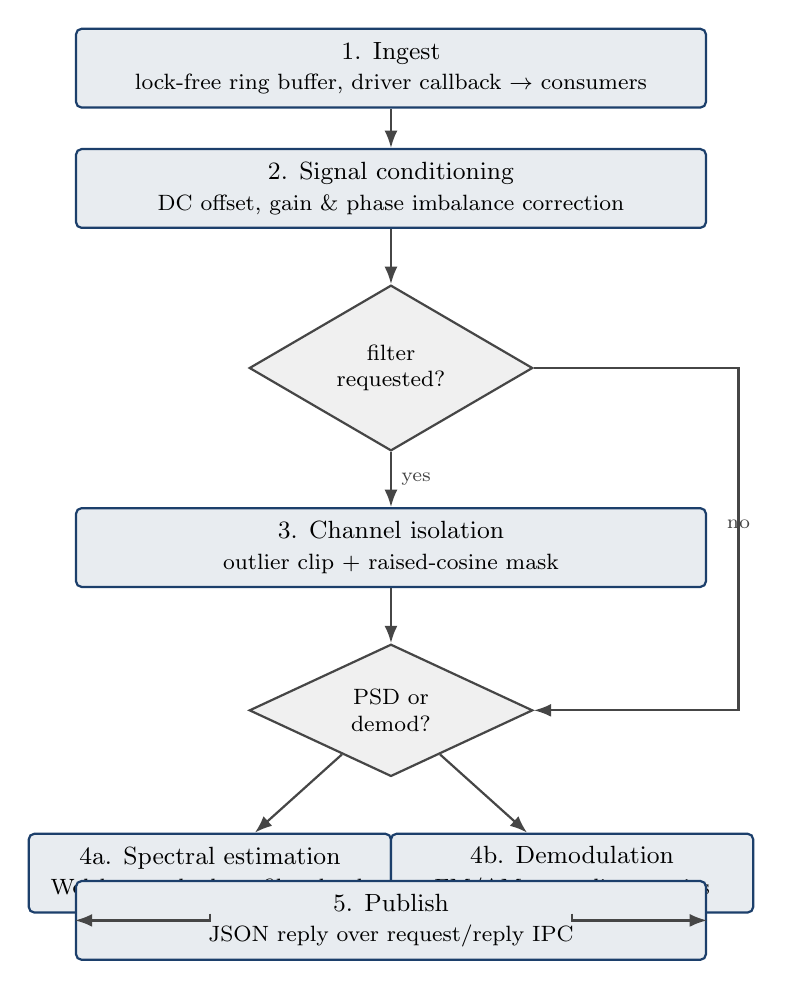
\begin{tikzpicture}[
    node distance=5mm,
    stage/.style={rectangle, rounded corners=2pt, draw=cplane, thick, fill=cplane!10,
                  minimum width=8cm, minimum height=1cm, align=center, font=\small},
    dec/.style={diamond, draw=neutralbox, thick, fill=neutralbox!8,
                minimum width=3.6cm, minimum height=1.1cm, align=center, font=\footnotesize,
                inner sep=1pt},
    arr/.style={-{Latex[length=2.2mm]}, thick, neutralbox}
]
\node[stage] (ingest) {1. Ingest\\{\footnotesize lock-free ring buffer, driver callback $\rightarrow$ consumers}};
\node[stage, below=of ingest] (cond) {2. Signal conditioning\\{\footnotesize DC offset, gain \& phase imbalance correction}};
\node[dec, below=7mm of cond] (filt) {filter\\requested?};
\node[stage, below=7mm of filt] (chan) {3. Channel isolation\\{\footnotesize outlier clip + raised-cosine mask}};
\node[dec, below=7mm of chan] (mode) {PSD or\\demod?};
\node[stage, below=7mm of mode, xshift=-2.3cm, minimum width=4.6cm] (psd) {4a. Spectral estimation\\{\footnotesize Welch \emph{or} polyphase filter bank}};
\node[stage, below=7mm of mode, xshift=2.3cm, minimum width=4.6cm] (demod) {4b. Demodulation\\{\footnotesize FM/AM + quality metrics}};
\node[stage, below=13mm of mode] (pub) {5. Publish\\{\footnotesize JSON reply over request/reply IPC}};

\draw[arr] (ingest) -- (cond);
\draw[arr] (cond) -- (filt);
\draw[arr] (filt) -- (chan) node[midway, right, font=\scriptsize] {yes};
\draw[arr] (filt.east) -- ++(2.6cm,0) |- (mode.east) node[near start, above, font=\scriptsize] {no};
\draw[arr] (chan) -- (mode);
\draw[arr] (mode) -- (psd);
\draw[arr] (mode) -- (demod);
\draw[arr] (psd) |- (pub);
\draw[arr] (demod) |- (pub);
\end{tikzpicture}
\caption{Conceptual DSP pipeline of the data plane, executed per acquisition request.}
\label{fig:dsp}
\end{figure}

\paragraph{Calibration as a distinct methodology.} Frequency reference error (PPM offset) is
determined not by a fixed factory value but by an on-device, three-stage search: a wideband
sweep identifies candidate strong signals, a pilot-tone detection stage (searching for the
stereo pilot characteristic of FM broadcast) identifies which candidate is a usable reference,
and a symmetry-based fine search around that reference estimates the frequency offset that
minimizes sideband asymmetry. The result is smoothed across runs and bounded by sanity limits
before being accepted, which protects the system against a single noisy measurement
corrupting the working calibration value. This is a self-calibrating methodology appropriate
for a device that cannot assume factory calibration remains valid over years of field
deployment and temperature variation.

\subsection{Control Plane / Orchestration}

The control plane is organized as a small set of independently scheduled responsibilities
rather than one monolithic loop:

\begin{itemize}[leftmargin=1.4em]
    \item \textbf{Realtime orchestration} polls the coordination server for on-demand
    configuration and relays it to the data plane, subject to the global state machine.
    \item \textbf{Campaign scheduling} treats longer-running, time-boxed measurement
    campaigns as a distinct concern from realtime polling: campaign definitions are
    fetched, persisted, and materialized into OS-level scheduled jobs, decoupling
    ``deciding what should run and when'' from ``actually running it.''
    \item \textbf{Status reporting} runs on a fixed timer, independent of acquisition
    activity, collecting host health telemetry (CPU, memory, disk, temperature, network
    reachability) and reporting it regardless of whether the sensor is currently acquiring.
    \item \textbf{Retry queueing} decouples successful local measurement from successful
    remote delivery: a measurement that cannot be uploaded (server unreachable, network
    outage) is persisted locally and retried on a separate schedule, rather than being lost
    or blocking the acquisition path.
\end{itemize}

This decomposition follows a general reliability methodology for unattended field devices:
each concern that can fail independently (acquisition, scheduling, reporting, delivery) is
given its own failure domain and its own recovery schedule, so that a fault in one does not
propagate into the others.

\subsection{GPS / LTE and RF Multiplexer Subsystem}
\label{sec:gpslte}

\undoc{The internal design of the GPS/LTE module and the RF multiplexer is not documented in
the material this reference is derived from.} Both are known to be present and operationally
used in the deployed system, but this reference deliberately does not speculate about their
internal implementation. What can be stated with confidence is their \emph{externally
observable interface contract}, inferred from the data the rest of the system consumes and
produces around them:

\begin{itemize}[leftmargin=1.4em]
    \item A GPS fix (latitude, longitude, altitude, and an associated timestamp) is
    available to the control plane and is reported upstream to the coordination server as
    a distinct telemetry type, separate from spectral data and status reporting.
    \item An antenna-port selector, constrained to a small fixed range of physical ports,
    is part of the realtime and campaign configuration contract, implying that RF-path
    selection (i.e., which physical antenna feeds the SDR for a given request) is
    externally configurable per request rather than fixed at deployment time.
    \item Time/location data of this kind is conventionally also used, in comparable
    systems, as an input to timestamp discipline and PPM-drift bookkeeping; whether this
    system uses it in that way, versus purely for geotagging, is \textbf{not established}
    by the available documentation and should not be assumed.
\end{itemize}

Figure~\ref{fig:gpsbox} represents this honestly: the subsystem is drawn as a boundary with a
known contract and an unknown interior.

\begin{figure}[H]
\centering
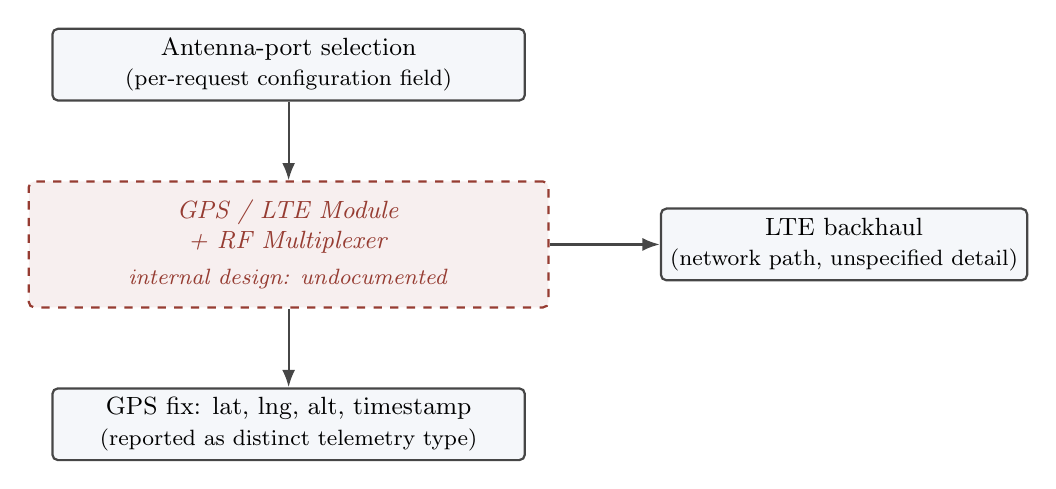
\begin{tikzpicture}[
    node distance=6mm,
    ifbox/.style={rectangle, rounded corners=2pt, draw=neutralbox, thick, fill=lightbg,
                  minimum width=6cm, minimum height=0.9cm, align=center, font=\small},
    gapbox2/.style={rectangle, rounded corners=2pt, draw=gapbox, thick, dashed, fill=gapbox!8,
                    minimum width=6.6cm, minimum height=1.6cm, align=center, font=\small},
    arr/.style={-{Latex[length=2.2mm]}, thick, neutralbox}
]
\node[ifbox] (in1) {Antenna-port selection\\{\footnotesize (per-request configuration field)}};
\node[gapbox2, below=10mm of in1] (gap) {\undoc{GPS / LTE Module}\\ \undoc{+ RF Multiplexer}\\[2pt]{\footnotesize\undoc{internal design: undocumented}}};
\node[ifbox, below=10mm of gap] (out1) {GPS fix: lat, lng, alt, timestamp\\{\footnotesize (reported as distinct telemetry type)}};
\node[ifbox, right=14mm of gap, minimum width=3.4cm] (out2) {LTE backhaul\\{\footnotesize (network path, unspecified detail)}};

\draw[arr] (in1) -- (gap);
\draw[arr] (gap) -- (out1);
\draw[arr] (gap.east) -- (out2.west);
\end{tikzpicture}
\caption{Interface-level view of the GPS/LTE/multiplexer subsystem. Only the boundary
contract is known; the interior is explicitly out of scope for this reference.}
\label{fig:gpsbox}
\end{figure}

% =====================================================================
\section{Data Flow Methodology}
% =====================================================================

Three data flows dominate normal operation. Each is shown as a vertical sequence in
Figures~\ref{fig:flow-realtime}--\ref{fig:flow-status}.

\begin{figure}[H]
\centering
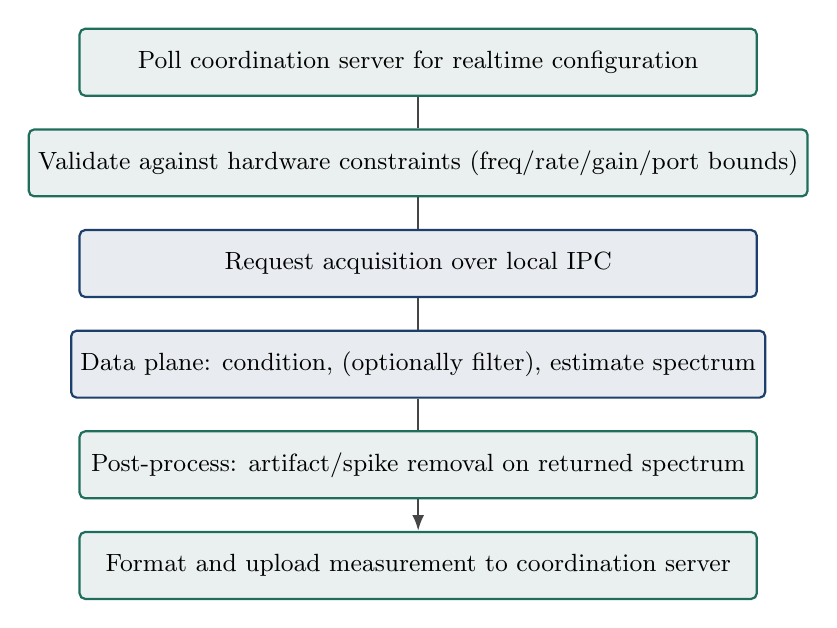
\begin{tikzpicture}[
    node distance=4mm,
    flowstep/.style={rectangle, rounded corners=2pt, draw=pyplane, thick, fill=pyplane!10,
                 minimum width=8.6cm, minimum height=0.85cm, align=center, font=\small},
    cstep/.style={flowstep, draw=cplane, fill=cplane!10},
    arr/.style={-{Latex[length=2mm]}, thick, neutralbox}
]
\node[flowstep] (s1) {Poll coordination server for realtime configuration};
\node[flowstep, below=of s1] (s2) {Validate against hardware constraints (freq/rate/gain/port bounds)};
\node[cstep, below=of s2] (s3) {Request acquisition over local IPC};
\node[cstep, below=of s3] (s4) {Data plane: condition, (optionally filter), estimate spectrum};
\node[flowstep, below=of s4] (s5) {Post-process: artifact/spike removal on returned spectrum};
\node[flowstep, below=of s5] (s6) {Format and upload measurement to coordination server};
\draw[arr] (s1)--(s2)--(s3)--(s4)--(s5)--(s6);
\end{tikzpicture}
\caption{Realtime acquisition flow.}
\label{fig:flow-realtime}
\end{figure}

\begin{figure}[H]
\centering
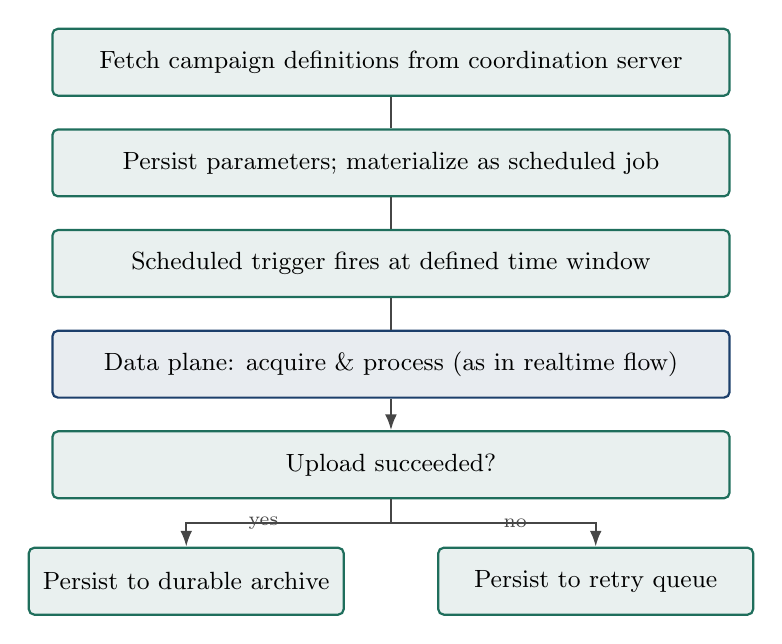
\begin{tikzpicture}[
    node distance=4mm,
    flowstep/.style={rectangle, rounded corners=2pt, draw=pyplane, thick, fill=pyplane!10,
                 minimum width=8.6cm, minimum height=0.85cm, align=center, font=\small},
    cstep/.style={flowstep, draw=cplane, fill=cplane!10},
    arr/.style={-{Latex[length=2mm]}, thick, neutralbox}
]
\node[flowstep] (c1) {Fetch campaign definitions from coordination server};
\node[flowstep, below=of c1] (c2) {Persist parameters; materialize as scheduled job};
\node[flowstep, below=of c2] (c3) {Scheduled trigger fires at defined time window};
\node[cstep, below=of c3] (c4) {Data plane: acquire \& process (as in realtime flow)};
\node[flowstep, below=of c4] (c5) {Upload succeeded?};
\node[flowstep, below=6mm of c5, xshift=-2.6cm, minimum width=4cm] (c6a) {Persist to durable archive};
\node[flowstep, below=6mm of c5, xshift=2.6cm, minimum width=4cm] (c6b) {Persist to retry queue};
\draw[arr] (c1)--(c2)--(c3)--(c4)--(c5);
\draw[arr] (c5.south) -- ++(0,-3mm) -| (c6a.north) node[near start, left, font=\scriptsize] {yes};
\draw[arr] (c5.south) -- ++(0,-3mm) -| (c6b.north) node[near start, right, font=\scriptsize] {no};
\end{tikzpicture}
\caption{Scheduled campaign acquisition flow.}
\label{fig:flow-campaign}
\end{figure}

\begin{figure}[H]
\centering
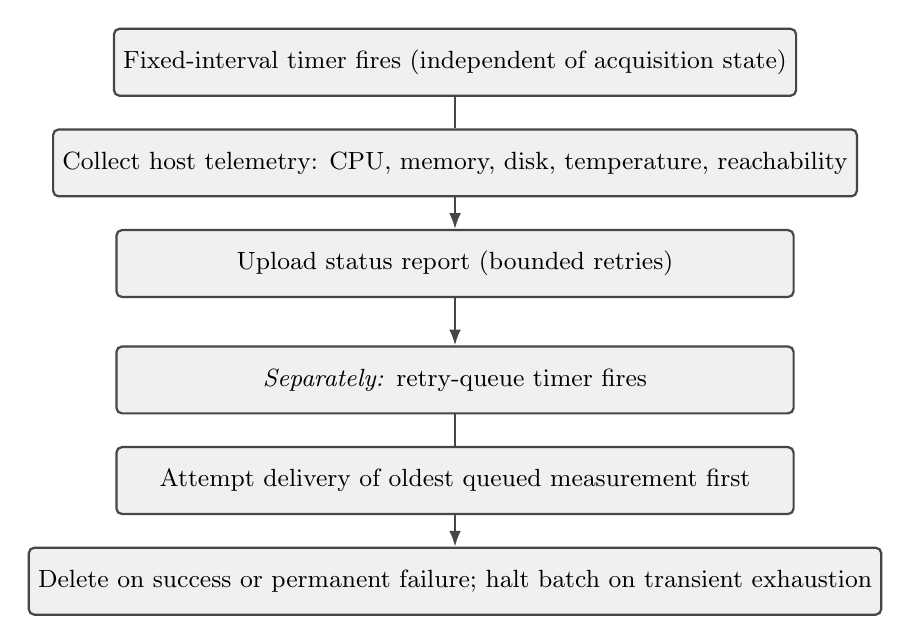
\begin{tikzpicture}[
    node distance=4mm,
    flowstep/.style={rectangle, rounded corners=2pt, draw=neutralbox, thick, fill=neutralbox!8,
                 minimum width=8.6cm, minimum height=0.85cm, align=center, font=\small},
    arr/.style={-{Latex[length=2mm]}, thick, neutralbox}
]
\node[flowstep] (t1) {Fixed-interval timer fires (independent of acquisition state)};
\node[flowstep, below=of t1] (t2) {Collect host telemetry: CPU, memory, disk, temperature, reachability};
\node[flowstep, below=of t2] (t3) {Upload status report (bounded retries)};
\node[flowstep, below=of t3, yshift=-2mm] (t4) {\textit{Separately:} retry-queue timer fires};
\node[flowstep, below=of t4] (t5) {Attempt delivery of oldest queued measurement first};
\node[flowstep, below=of t5] (t6) {Delete on success or permanent failure; halt batch on transient exhaustion};
\draw[arr] (t1)--(t2)--(t3);
\draw[arr] (t3)--(t4);
\draw[arr] (t4)--(t5)--(t6);
\end{tikzpicture}
\caption{Status reporting and retry-queue flow (both timer-driven, independent of acquisition).}
\label{fig:flow-status}
\end{figure}

% =====================================================================
\section{Concurrency and State Model}
\label{sec:statemachine}
% =====================================================================

Acquisition-related concurrency is governed by a single global state machine rather than
fine-grained locking. This is a deliberate simplification: because the underlying hardware
resource (the SDR) is strictly single-owner, coarse mutual exclusion at the level of
\emph{intent} (``what kind of activity is the node currently committed to'') is sufficient and
easier to reason about than lock-based coordination deep inside the acquisition path.

\begin{figure}[H]
\centering
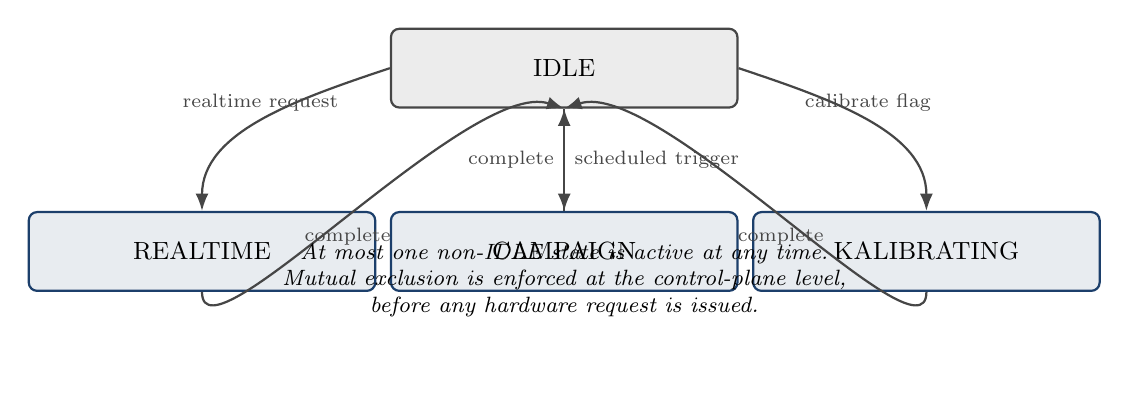
\begin{tikzpicture}[
    node distance=13mm,
    st/.style={rectangle, rounded corners=3pt, draw=cplane, thick, fill=cplane!10,
               minimum width=4.4cm, minimum height=1cm, align=center, font=\small},
    idle/.style={st, draw=neutralbox, fill=neutralbox!10},
    arr/.style={-{Latex[length=2.2mm]}, thick, neutralbox}
]
\node[idle] (idle) {IDLE};
\node[st, below=of idle, xshift=-4.6cm] (rt) {REALTIME};
\node[st, below=of idle] (camp) {CAMPAIGN};
\node[st, below=of idle, xshift=4.6cm] (kal) {KALIBRATING};

\draw[arr] (idle.west) .. controls +(-1.2,-0.4) and +(0,1.0) .. (rt.north) node[midway, above, font=\scriptsize] {realtime request};
\draw[arr] (rt.south) .. controls +(0,-1.0) and +(-1.2,0.4) .. (idle.south) node[midway, below, font=\scriptsize] {complete};

\draw[arr] (idle) -- (camp) node[midway, right, font=\scriptsize] {scheduled trigger};
\draw[arr] (camp) -- (idle) node[midway, left, font=\scriptsize] {complete};

\draw[arr] (idle.east) .. controls +(1.2,-0.4) and +(0,1.0) .. (kal.north) node[midway, above, font=\scriptsize] {calibrate flag};
\draw[arr] (kal.south) .. controls +(0,-1.0) and +(1.2,0.4) .. (idle.south) node[midway, below, font=\scriptsize] {complete};

\node[below=16mm of idle, align=center, font=\footnotesize\itshape] {At most one non-IDLE state is active at any time.\\Mutual exclusion is enforced at the control-plane level,\\before any hardware request is issued.};
\end{tikzpicture}
\caption{Global acquisition state machine. Transitions out of IDLE are gated by whichever
trigger arrives first; the state machine itself is the mechanism preventing two acquisition
intents from being active simultaneously.}
\label{fig:statemachine}
\end{figure}

% =====================================================================
\section{Reliability and Fault-Tolerance Methodology}
% =====================================================================

Table~\ref{tab:reliability} summarizes the failure modes the architecture explicitly
anticipates and the corresponding design pattern used to contain each one. This mapping is
useful as a checklist when evaluating whether a proposed change preserves the system's
reliability posture.

\begin{table}[H]
\centering
\small
\begin{tabular}{@{}p{4.6cm}p{4.6cm}p{5cm}@{}}
\toprule
\textbf{Failure mode} & \textbf{Design pattern applied} & \textbf{Layer} \\
\midrule
SDR/USB disconnect or register-level fault & Session health check before each use; bounded-attempt device reopen & Data plane \\
Stalled IPC request/reply handshake & Destroy and recreate the socket, resetting protocol state & Both planes (paired) \\
Stale samples in acquisition buffer & Discard-to-head before each request (request-scoped capture) & Data plane \\
Coordination-server unreachable & Persist-and-retry queue, independent schedule from acquisition & Control plane \\
Process crash / unresponsive process & Restart-always service supervision with singleton locking & OS / service layer \\
Power loss mid-write to shared state & Write-temp $\rightarrow$ fsync $\rightarrow$ atomic replace, under advisory lock & Both planes (paired) \\
CPU/thermal overload from rapid requests & Configurable inter-request pacing (``cooldown'') & Data plane \\
Idle hardware power/thermal draw & Lazy hardware open; idle timeout closes device & Data plane \\
Concurrent conflicting acquisition intents & Global mutually-exclusive state machine & Control plane \\
Blocked thread delaying shutdown & Cooperative cancellation checked on short polling interval & Both planes \\
Frequency reference drift over time/temperature & On-device self-calibration with outlier-bounded smoothing & Data plane \\
\bottomrule
\end{tabular}
\caption{Failure modes anticipated by the architecture and the corresponding mitigation pattern.}
\label{tab:reliability}
\end{table}

% =====================================================================
\section{Comparative Positioning Relative to the State of the Art}
% =====================================================================

Table~\ref{tab:sota} situates the system, at a conceptual level, against the general class of
distributed low-cost spectrum-sensing platforms exemplified by ElectroSense and its
successors, without claiming precise, sourced performance figures for either side.

\begin{table}[H]
\centering
\small
\begin{tabular}{@{}p{3.6cm}p{5.4cm}p{5.4cm}@{}}
\toprule
\textbf{Dimension} & \textbf{Canonical crowdsourced platforms\newline(e.g., ElectroSense-class)} & \textbf{This system} \\
\midrule
Deployment model & Open, crowdsourced; volunteer-hosted nodes & Regulator-operated; scheduled campaigns \\
SDR front end & RTL-SDR-class, often with an auxiliary up/down-converter for multi-GHz reach & HackRF One, native continuous coverage into the low-GHz range \\
Edge DSP scope & Evolved from cloud-side FFT toward increasing on-device processing (successor generations) & On-device compensation, filtering, PSD estimation, and demodulation from the outset \\
Backend interaction & Public/open API, crowdsourced backend & Single authoritative coordination server, private API \\
Acquisition modes & Primarily continuous/streaming sensing & Explicit dual mode: on-demand realtime \emph{and} scheduled, time-boxed campaigns \\
Ancillary sensing & GPS commonly used for time sync & GPS/LTE module present; exact internal role not established (Section~\ref{sec:gpslte}) \\
\bottomrule
\end{tabular}
\caption{Conceptual positioning against the general class of distributed spectrum-sensing platforms.}
\label{tab:sota}
\end{table}

The broader field trend --- pushing DSP work from a centralized backend toward the sensing
edge as embedded compute capacity grows --- is directly reflected in this system's decision
to perform IQ compensation, filtering, spectral estimation, artifact removal, and even
self-calibration entirely on-node, with the backend receiving already-processed spectral and
telemetry data rather than raw samples.

% =====================================================================
\section{Limitations and Open Questions}
% =====================================================================

\begin{itemize}[leftmargin=1.4em]
    \item \textbf{GPS/LTE and multiplexer internals are undocumented.} As stated in
    Section~\ref{sec:gpslte}, only the interface contract is known. A complete architecture
    reference would require either the source documentation for this subsystem or direct
    inspection of its implementation.
    \item \textbf{Single point of hardware failure.} The architecture assumes exactly one
    SDR front end; there is no redundant RF path, so a permanent hardware fault removes the
    node from service until physically serviced.
    \item \textbf{Permissive configuration parsing.} The control-plane/data-plane
    configuration contract is deliberately permissive (unrecognized fields ignored,
    malformed input falls back to defaults) to tolerate an imperfect network link. This is
    a reasonable trade-off for availability but means a malformed campaign definition could
    silently run with unintended parameters rather than failing loudly; this may warrant an
    explicit validation-failure signal in future iterations.
    \item \textbf{Authentication and transport security} of the remote API were out of scope
    for the documentation this reference was derived from and are not characterized here.
\end{itemize}

% =====================================================================
\section{Conclusion}
% =====================================================================

The sensor node's architecture follows an edge-first methodology consistent with the broader
trajectory of distributed spectrum-sensing research: minimize backhaul dependence by
performing signal conditioning, spectral estimation, artifact removal, and self-calibration
on-device; isolate the real-time acquisition path from supervisory logic through a strict
data-plane/control-plane split; and favor coarse-grained, easily-reasoned-about concurrency
control (a global state machine, request-scoped capture, atomic persistence) over fine-grained
locking. The result is a node designed to operate unattended, recover automatically from the
transient failure modes typical of field deployment, and support both on-demand and scheduled
regulatory measurement workflows. The principal open gap in this reference is the internal
design of the GPS/LTE and RF-multiplexer subsystem, which should be the subject of a follow-up
documentation pass once its implementation is available for review.

\end{document}
